\section{Cartes Lothaire}
\begin{figure}[H]
    \center
    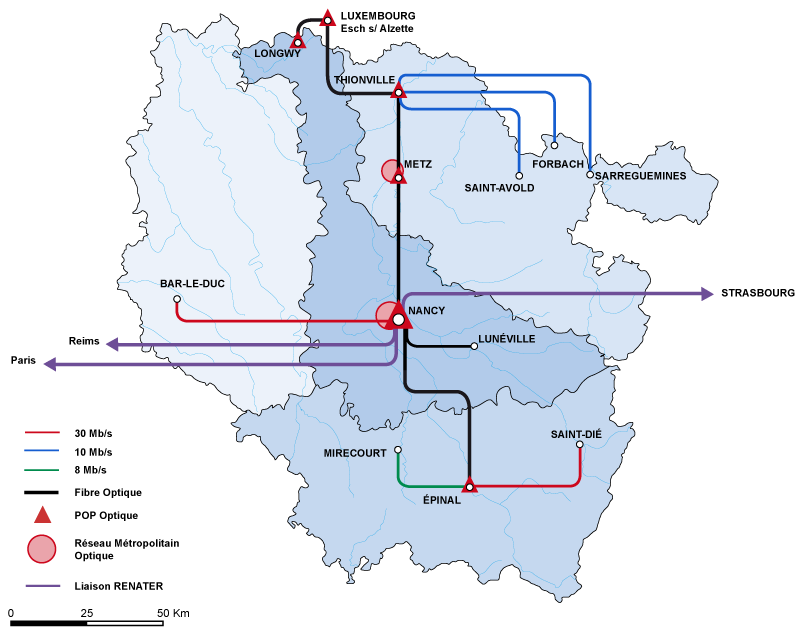
\includegraphics[width=1\textwidth]{carte_lothaire.png}
    \label{fig:imagereseaulothaire1}
    \caption{Cartographie des interconnexions}
\end{figure}
\begin{figure}[H]
    \center
    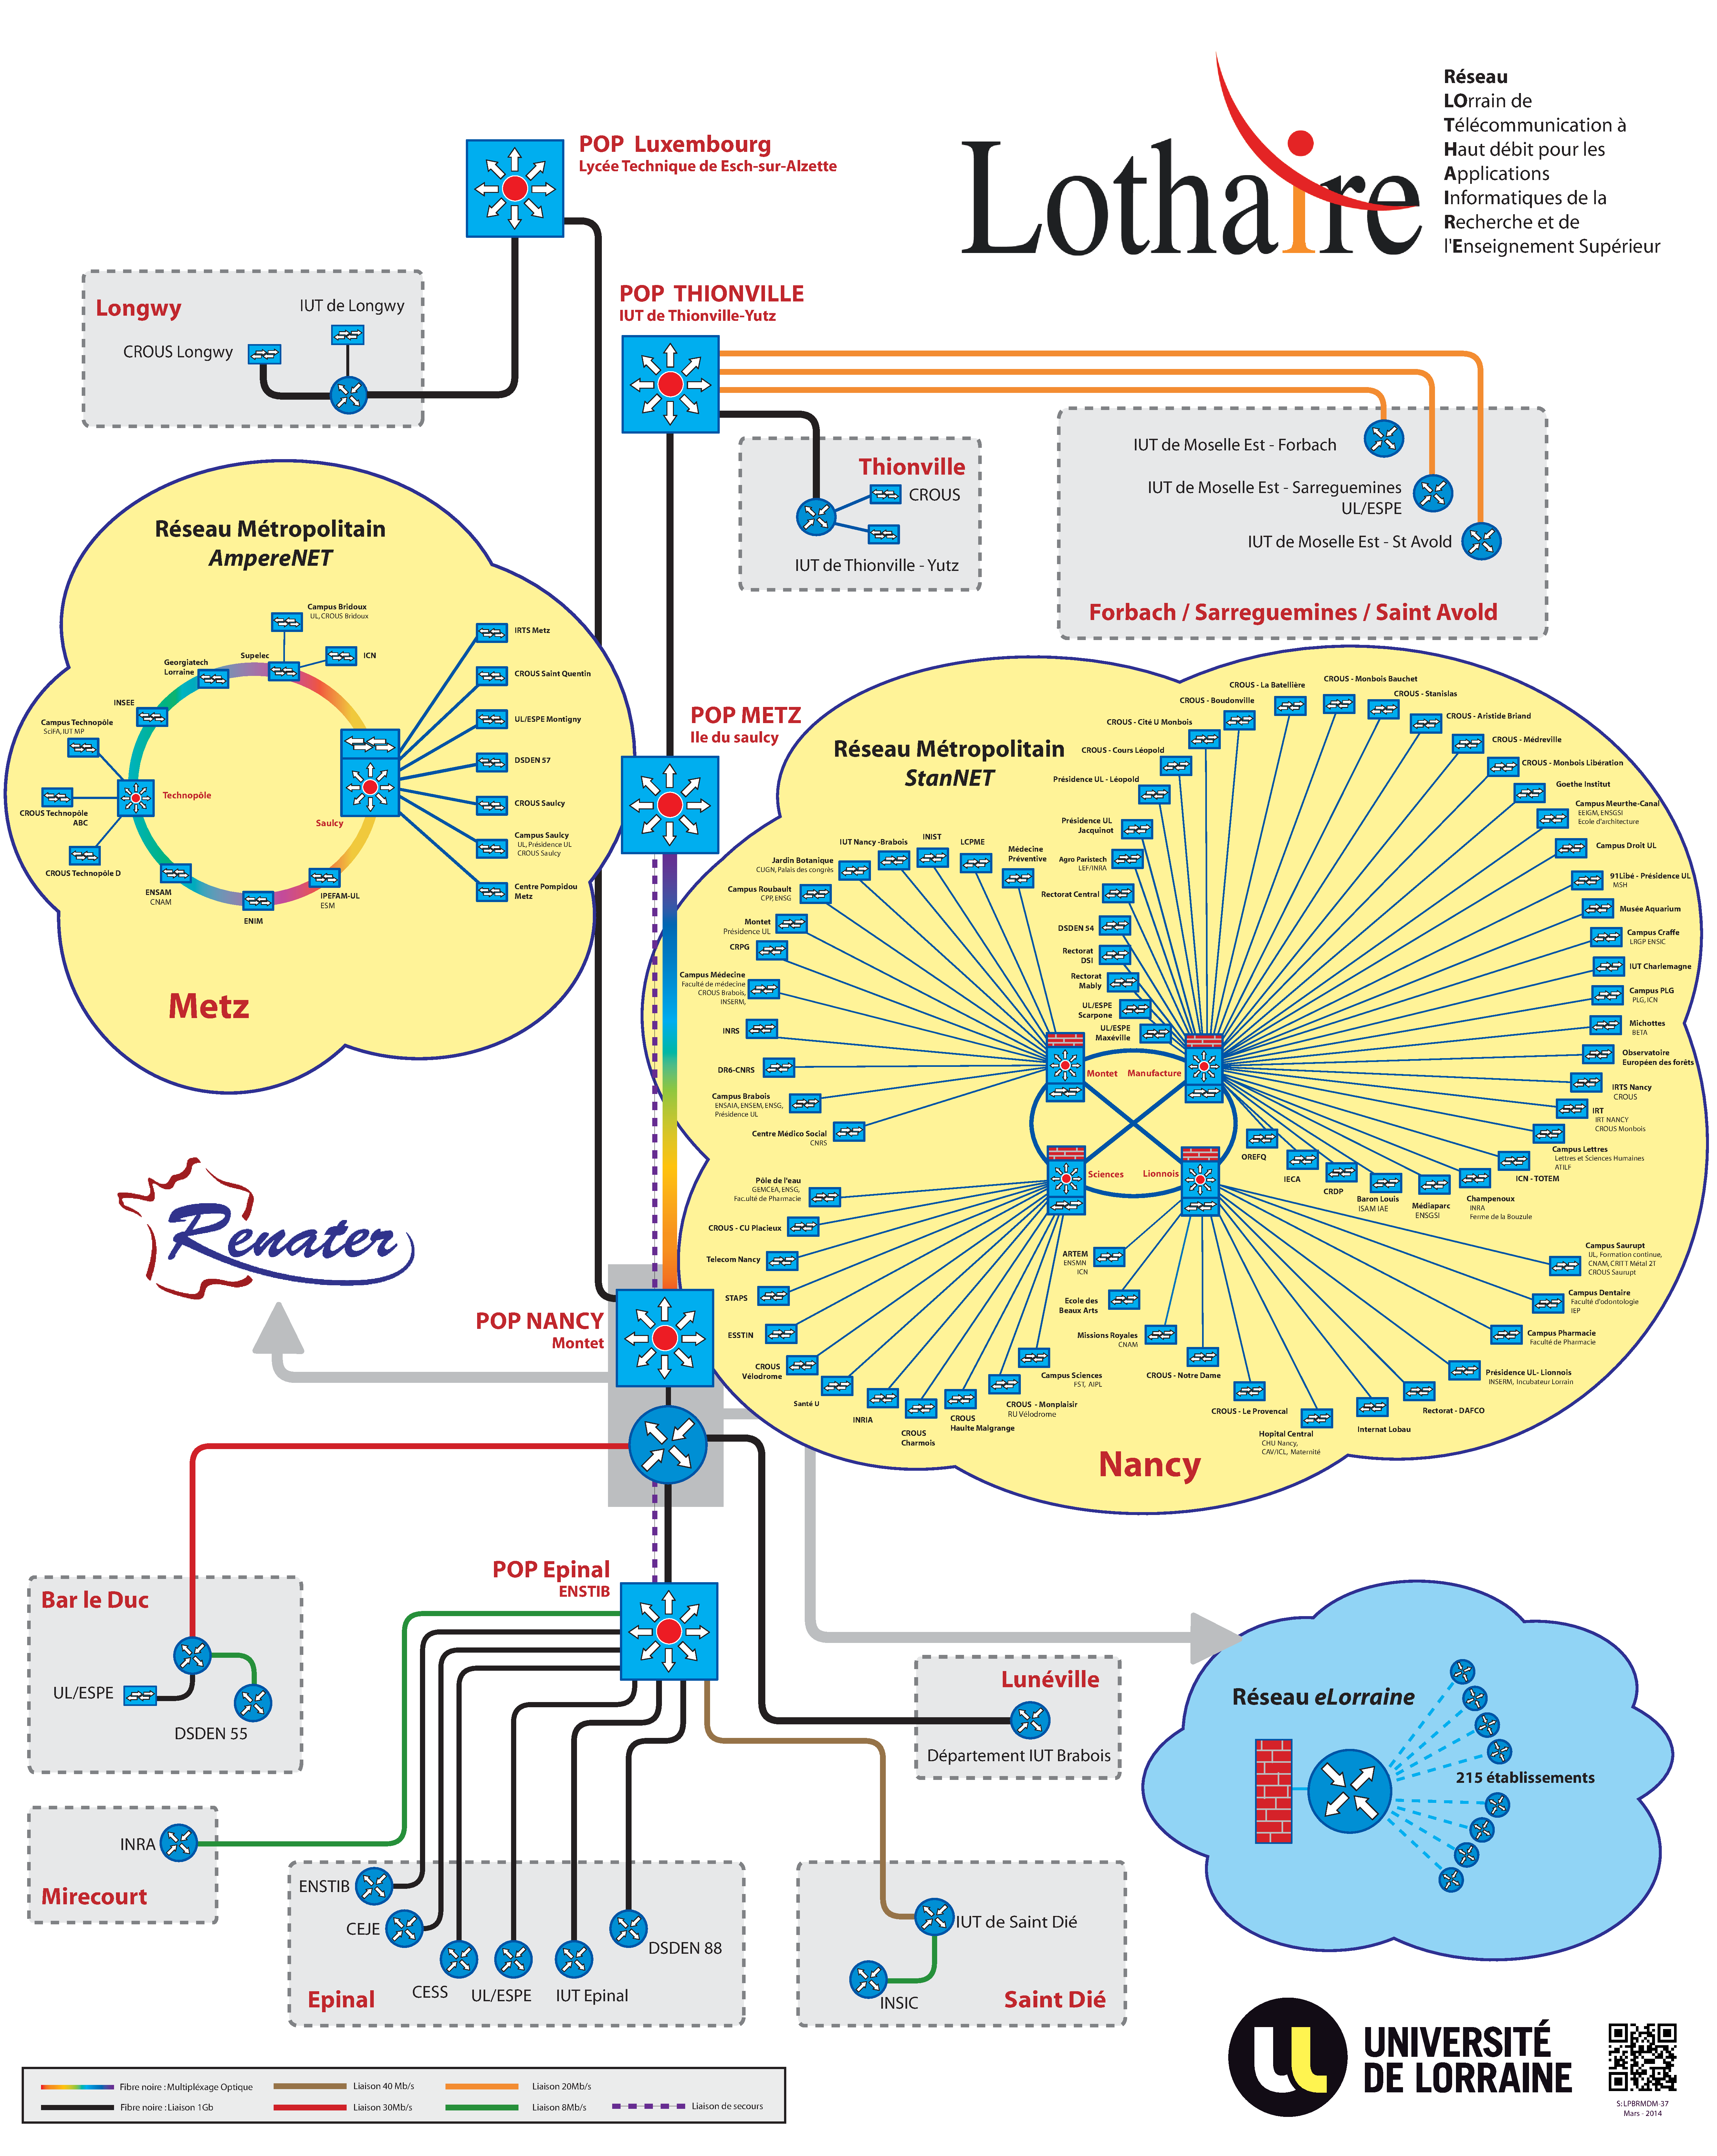
\includegraphics[width=1\textwidth]{poster-lothaire.pdf}
    \label{fig:imagereseaulothaire2}
    \caption{Représentation du réseau Lothaire}
\end{figure}


\section{Images Kibana}
\begin{figure}[H]
\center
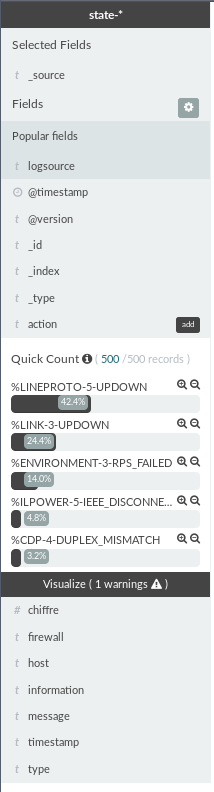
\includegraphics[width=0.4\textwidth,height=0.8\textheight]{kibanatuto/rap/4.png}
\label{fig:kibanatuto4}
\caption{Le tableau des champs}
\end{figure}
\paragraph{}
\begin{figure}[H]
\center
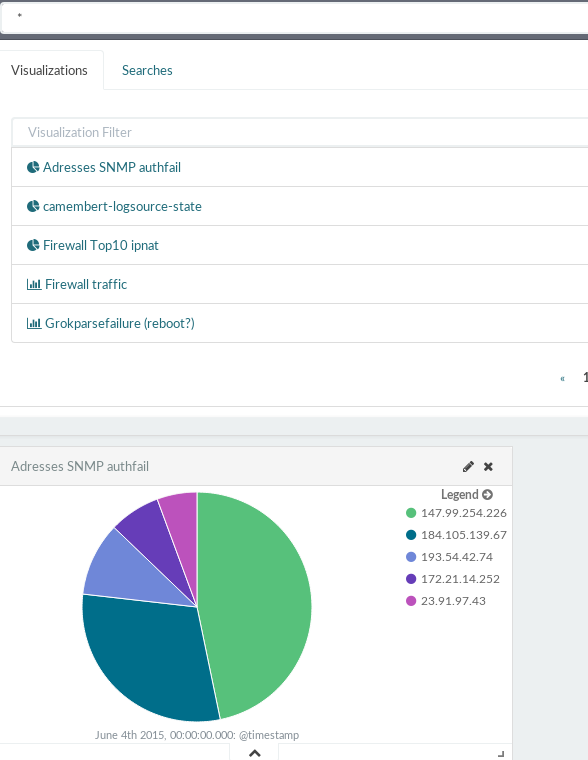
\includegraphics[width=0.8\textwidth]{kibanatuto/rap/17.png}
\label{fig:kibanatuto10}
\caption{Choix des visualisations}
\end{figure}
\paragraph{}
\begin{figure}[H]
\center
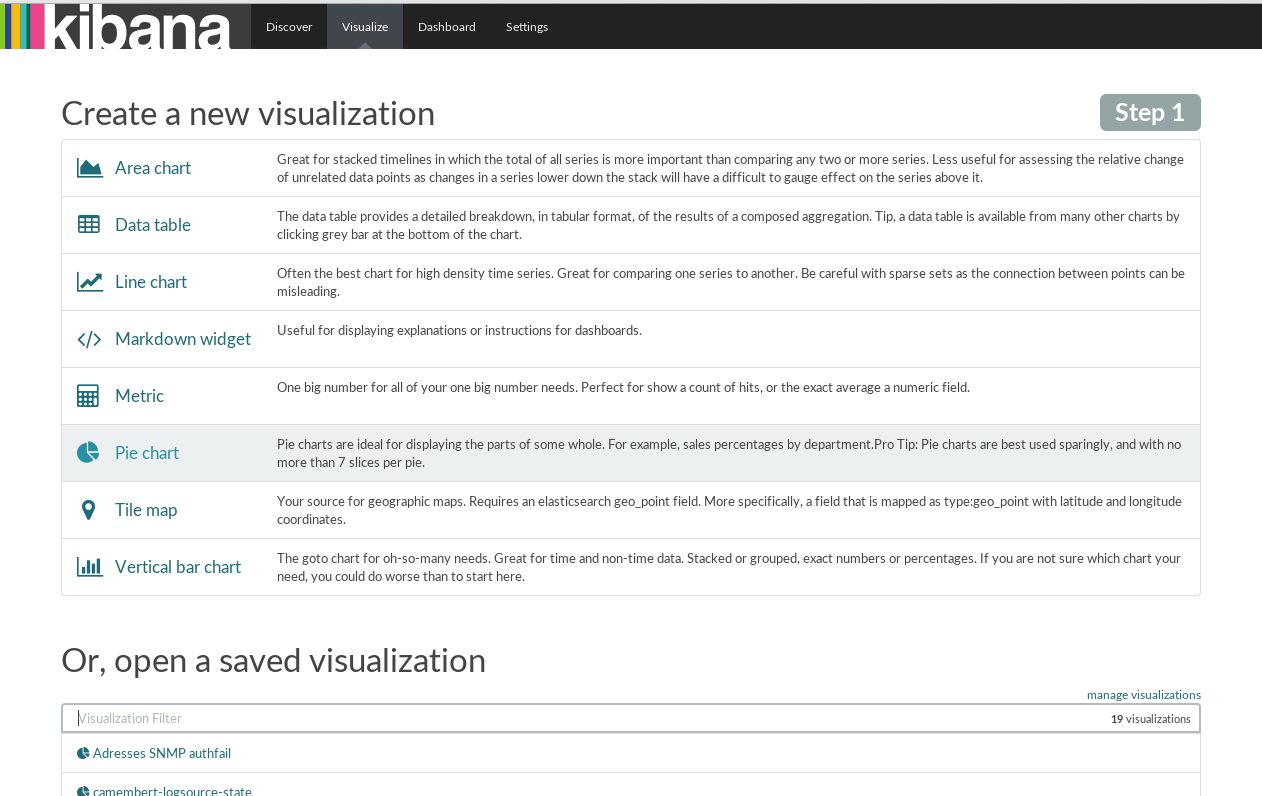
\includegraphics[width=1\textwidth]{kibanatuto/rap/10.png}
\label{fig:kibanatuto7}
\caption{Visualisations possibles}
\end{figure}
\paragraph{}
\begin{figure}[H]
\center
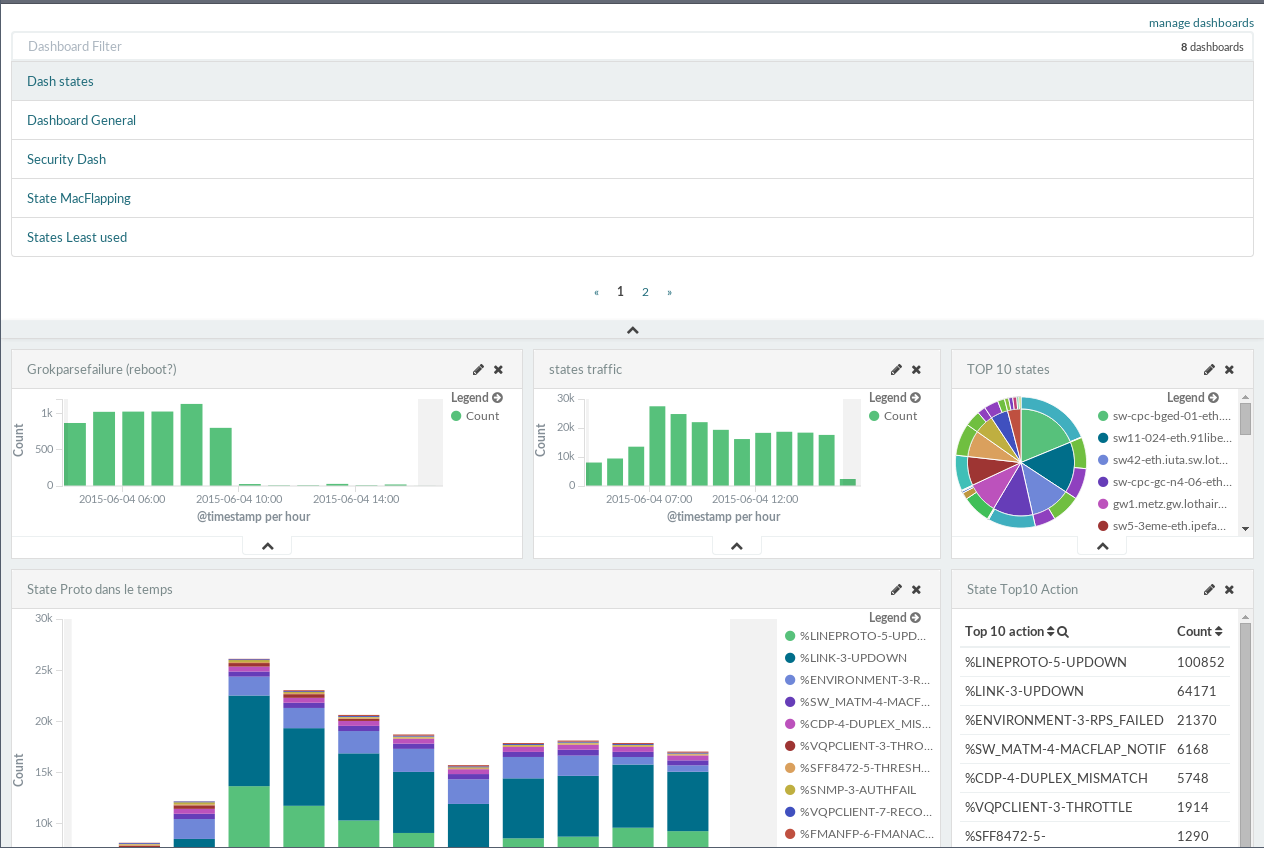
\includegraphics[width=1\textwidth]{kibanatuto/rap/19.png}
\label{fig:kibanatuto12}
\caption{Dashboard plus avancé}
\end{figure}

\section{Statistiques Munin}
\begin{figure}[H]
\center
\includegraphics[width=1\textwidth]{munin/elk2cpu-month2.png}
\label{fig:elk2cpu}
\caption{Consommation CPU effective mensuel d'Elk2, en bleu\ldots}
\end{figure}
Ne vous esquintez pas les yeux, le bleu est pratiquement indiscernable.

\begin{figure}[H]
\center
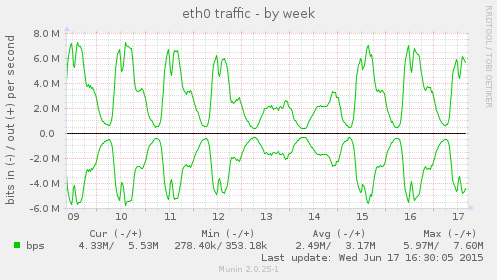
\includegraphics[width=1\textwidth]{munin/elk2if_eth0-week.png}
\label{fig:elk2eth0}
\caption{Bande passante Up et Down de Elk2}
\end{figure}
\begin{figure}[H]
\center
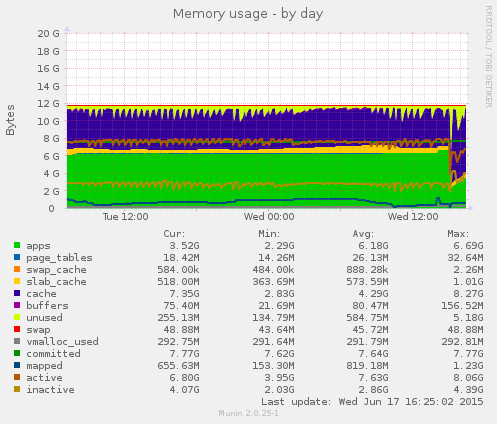
\includegraphics[width=0.8\textwidth]{munin/elk1memory-day.png}
\label{fig:elk1memory}
\caption{Utilisation RAM Elk1}
\end{figure}
La ligne orange représente la RAM effectivement utilisée, la zone bleue la mémoire virtuelle.
\begin{figure}[H]
\center
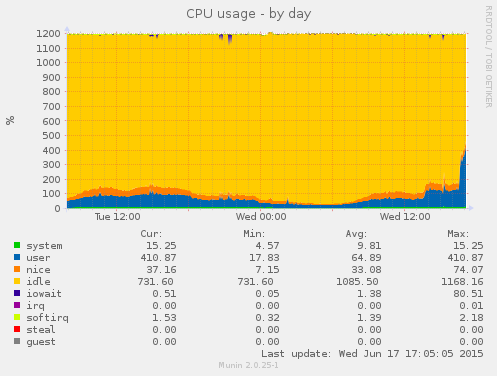
\includegraphics[width=0.8\textwidth]{munin/elk1cpu-day.png}
\label{fig:elk1cpu}
\caption{Utilisation CPU Elk1}
\end{figure}
